
{  % 單一語音離散表徵與音位的關係

  HuBERT \cite{hsu_hubert_2021, hsu_hubert_2021-2} 和 Wav2vec 2.0 \cite{baevski2020wav2vec} 等語音基石模型的成功,不僅在語音任務上達到了前所未有的表現,還促進了語音表徵離散化的發展。由此產生的「無文字(Textless)」架構 \cite{noauthor_textless_2021, lakhotia_generative_2021, lakhotia_generative_2021-1},讓人們在處理語音訊號時,有了連續表徵以外的新選擇。離散形式的表徵可以直接應用文字領域發展的技術,如機器翻譯、生成式模型等,為語音技術帶來新的突破。另一方面,基於離散「符記(Token)」的共同形式,離散語音表徵可以更好的整合文字資料,促成多模態領域的發展。跨模態離散表徵的成功,甚至驅使影像領域也開始發展離散表徵,\jeffcomment{\textcolor{yellow}{(要確認一下「開始」嗎?)}}如探討唇語的 AV-HuBERT \cite{shi2021learning} 等等,展現了離散表徵在資料處理上的優勢。

        此外,除了技術的角度切入,這樣的技術也可以探討離散語音表徵成功背後的可能因素,以及它們與語言學對人類語音理解之間的差異,甚至是進一步利用這些技術協助更細緻的探討人類的語音現象。因此,原先在連續語音表徵上的語音學分析,也開始關注離散表徵在多大程度上能描述語音現象,將其列入考量,成為除了連續語音特徵和時頻譜之外的另一個選擇。

}  % 單一語音離散表徵與音位的關係

\section{相關研究}  

\subsection{無文字與離散語音表徵}

  自 HuBERT 帶起的研究之後,出現了愈來愈多離散表徵相關的研究\cite{10097097, abdullah23_interspeech, chang_exploration_2023, liu2024dinosr, zhang2024speechtokenizer, huang2023repcodec} 。它們在提出自己的離散表徵時,也會採取 HuBERT 的衡量方式,來驗證這些離散單元與語音中的內容及人類對語音的詮釋之間,具有一定程度的相關性,並從資訊理論(Information Theory)的角度,證明這些離散單元確實具備區分不同語音資訊的能力。

\subsection{語音學分析}

  由於語音處理本身最終是針對人類語音,因此有一群研究者通過對人類語音的理解,將這些知識應用在分析模型如何對語音訊號建構表徵之上\cite{deseyssel22_interspeech, wells_phonetic_2022, 10097097, abdullah23_interspeech} 。基於這些作品對語音離散表徵的興趣和探討,本論文也先透過過往幾個常用來分析語音表徵的方式,特別是 HuBERT \cite{hsu_hubert_2021-2} 提出的標準進行初步的分析。


\section{衡量方式}

  本次研究主要探討純度(Purity)、熵(Entropy)和相互資訊(Mutual Information,MI)等指標,這些指標在 HuBERT 中被採用 \cite{hsu_hubert_2021, hsu_hubert_2021-2},用以比對機器學習過程中得到的虛擬標註與人類標註之間的相關性(Correlation)。以下對各標準進行詳細解釋:

        不論是何種語音基石模型,語音表徵的基本單位是音框(Frame)。因此一段語句(Utterance)的語音離散單元被表示為 $[y_1, \cdots\cdots, y_T]$。其中 $T$ 是該段語句的音框總數。對於該段語句,若給予一段在音框上對齊的音素標註(Phonetic Label) $[z_1, \cdots\cdots, z_T]$,此時我們可以將離散單元與標註之間配對的出現次數,寫為一個雙變數的共同分佈(Joint Distribution)
\begin{align}
    p_{yz} = \frac{\sum^T_{t=1}[{y_t = i \wedge z_t = j}]}{T}
\end{align}

其中 $i$ 是第 $i$ 個音位類別,而 $j$ 指編號為$j$的離散單元。兩個變數的邊際機率(Marginal Probability)分別為
\begin{align}
    p_z(j) & =\sum_i{p_{yz}(i, j)} \\
    p_y(i) & =\sum_j{p_{yz}(i, j)}
\end{align}
因此,對於每一個音位 $i$ 而言,這個音位最可能的對應離散單元為
\begin{align}
    z^\ast(i) = \arg\max_j p_{yz}(i, j)
\end{align}
與之相對應的,對於每一個離散單元的類別 $j$ 則可以找到機率最高的音位
\begin{align}
    y^\ast(j) = \arg\max_i p_{yz}(i,j)
\end{align}
透過這些定義,以下分節介紹將要用來分析的指標:

\subsection{純度}

  本指標考慮音位和離散單元兩個序列之間對應的最高機率,因此從音位與離散單元的角度出發,可以得到以下兩項數據:

\paragraph{音位純度(Phoneme Purity)}\hfill \break
%
        考慮每個離散單元對應的音位中,最高機率音位的機率,表示為
\begin{align}
    \mathbb{E}_{p_z(j)}\left[p_{y|z}(y^*(j)|j) \right]
\end{align}
此指標表示該單元是否對其對應的音位有足夠的代表性。

\paragraph{分群純度(Cluster Purity)}\hfill \break
%
        與音位純度相對,改以每個音位的角度,考慮對應單元類別的機率
\begin{align}
    \mathbb{E}_{p_y(i)}\left[p_{z|y}(z^*(i)|i) \right]
\end{align}
        由於離散表徵進行分群演算法時的類別數是一項超參數(Hyperparameter),且通常離散單元的分群數量會比音位多,因此該統計數據本身不直接具有語音學的解釋意義,而且在分群數量很多時其數值會顯著下降。然而該指標在考量音位純度時必須一併考慮,因為當分群數非常多時,分群純度過低暗示離散單元做不到歸納音位類別的效果,使得音位純度失去其意義。一個極端的情形是每一個音框都給予不同的離散單元編號,如此音位純度可以達到100\%。

\subsection{熵和相互資訊}

  除了純度提供「最高機率」的對應關係,根據 HuBERT 論文 \cite{hsu_hubert_2021-2} 中的分析方式,我們也可以從資訊理論的角度,觀察兩個序列的熵和相互資訊。

\paragraph{熵(Entropy)} \hfill \break
%
  熵的定義按照資訊理論,衡量兩個序列中標籤類別出現機率的不確定性(Uncertainty),公式寫作:
\begin{align}
    H(y) & = \sum_i{p_y(i)\log p_y(i)} \\
    H(z) & = \sum_j{p_z(j)\log p_z(j)}
\end{align}
其中 $H(y)$ 和 $H(z)$ 分別為音位和離散單元的熵,數值愈高分別表示各種音位和離散單元出現的機率愈平均。

\paragraph{以音位標準化之相互資訊(Phone-normalized Mutual Information,PNMI)}\hfill \break
%
  本數據以「觀察到某一個離散單元,能降低多少音位標註的不確定性」,定義該離散單元的出現背後提供了多少音位的資訊。公式寫為:
\begin{align}
    \frac{I(y;z)}{H(y)} & =\cfrac{\sum_i \sum_j p_{yz}(i, j) \log \cfrac{p_{yz}(i, j)}{p_y(i)p_z(j)}}{\sum_i p_y(i) \log p_y(i)} \\
                        & =\frac{H(y)-H(y|z)}{H(y)}                                                                              \\
                        & =1-\frac{H(y|z)}{H(y)}
\end{align}
        該項數據愈高,表示離散單元的分群愈能提供語音音位的資訊,是一個品質更好的分群結果。由於離散單元是否能夠正確對應到音位才是人們所關心的問題,因此與純度不同,只以音位的角度出發,而不考慮以離散單元分群的角度。

\section{語音學的音位分類(Phoneme Type)}

  除了單一音位本身的特性以外,由於音位之間存在相似的特徵,可以分成幾個組別。這裡依照希氏(Sicherman) \cite{10097097}、阿氏(Abdullah)\cite{abdullah23_interspeech} 等前作的分組方式,對英語的音位進行分類並合併比對數據,觀察這些離散單元是否有擷取到相似的發聲特徵,而不單純只是把音位分成約 50 類完全獨立的標籤。以下簡介六個音位組別:
        
        \begin{itemize}
            \item 塞音(Plosive):以完全阻塞氣流的方式發音的音位,包含 /p/、/b/、/t/、/d/、/k/、/g/ 六種
            \item 擦音(Fricative):藉由在口腔中形成的縫隙,使氣流通過時摩擦形成的發音,包含 /f/、/v/、/s/、/z/、/\textesh/ (sh)、/\textyogh/ (如「garage」的 「-ge」)、/θ/ (無聲的 th)、/ð/ (有聲的 th)、/h/ 九種
            \item 塞擦音(Affricate):由塞音和同部位的擦音同時發出的輔音,英語中只有 /t\textesh/ 和 /d\textyogh/ 兩種,即 ch 和 j 的發音
            \item 鼻音(Nasal):使氣流通過鼻腔形成的聲音,有 /m/、/n/、/ŋ/ (ng) 三種
            \item 近音(Approximant):又稱半元音,為介於元音和輔音之間的聲音,有 /j/ (為 y 作為輔音時的發音)、/r/、/l/、/w/
            \item 元音(Vowel):可自成音節的音位,包含發音位置固定的單元音(Monophthong)和會移動的的雙元音(Diphthong),通常以 a、e、i、o、u 字母產生的聲音皆屬於此類別
        \end{itemize}
        
        透過將音位分組後,形成新的語音標註,並重新分析統計指標,觀察在純度等數據是否顯示離散單元與語音的發音方式具有更明確的關聯性。

\section{[[ Write here! ]]}


{
%%%%%%%%%% write here
}  % 單一語音離散表徵與音位的關係

\setcounter{section}{4}
\section{實驗集與分析模型}

  本研究的分析對象參考無文字架構 \cite{noauthor_textless_2021, lakhotia_generative_2021, lakhotia_generative_2021-1} 的研究,
採用論文中提及的四種語音表徵,簡述如下:

\begin{itemize}
    \item CPC:卷積式編碼器 + 遞迴式預測器,以對比式學習訓練。表徵來自預測器的中間層,每 10 毫秒提取一個向量表徵作為音框
    \item Wav2vec 2.0:卷積式編碼器 + 轉換器預測器,以對比式學習訓練。表徵來自轉換器第 14 層,每 20 毫秒作為一個音框
    \item HuBERT:卷積式編碼器 + 轉換器預測器,以預測式學習訓練,其訓練目標為 K-平均分群演算法的結果,透過遮蔽語言模型的方式訓練。表徵來自轉換器第 6 層,每 20 毫秒作為一個音框
    \item LogMel:為 80 維對數梅爾時頻譜的聲學特徵,在此作為比較基線(Baseline)。音框寬度為 10 毫秒
\end{itemize}

        我們使用該論文\textcolor{red}{(哪一篇?)}釋出之預訓練模型與 K-平均量化模型。預訓練模型細節詳述於 \cite{lakhotia_generative_2021-1} 中,量化模型則是該篇論文透過公開的 LibriSpeech 資料集 \cite{panayotov_librispeech_2015} 中 train-clean-100 訓練集,獲取語音表徵後執行 K-平均分群演算法所得,並釋出群數為 50、100 和 200 的三個版本。

        本論文以 LibriSpeech train-clean-100 作為分析對象,將語音語料庫的語音資料經過四個模型獲取連續表徵後,再經過量化模型得到完全由離散單元組成的「虛擬文字」語料。

        本論文針對語音學的音位標註,透過強迫對齊器(Forced-aligner)\footnote{https://github.com/MontrealCorpusTools/Montreal-Forced-Aligner}的英語預訓練模型,從語料庫的文字轉寫取得語音資料的音位標註與對應的時間範圍。最後透過語音表徵各自的時間解析度生成以音框為單位的音位標註語料。最後將兩者對語音資料集進行音位標註相關性的分析。


\setcounter{section}{4}

\section{分析結果 (New)}

{



\begin{figure}\centering
    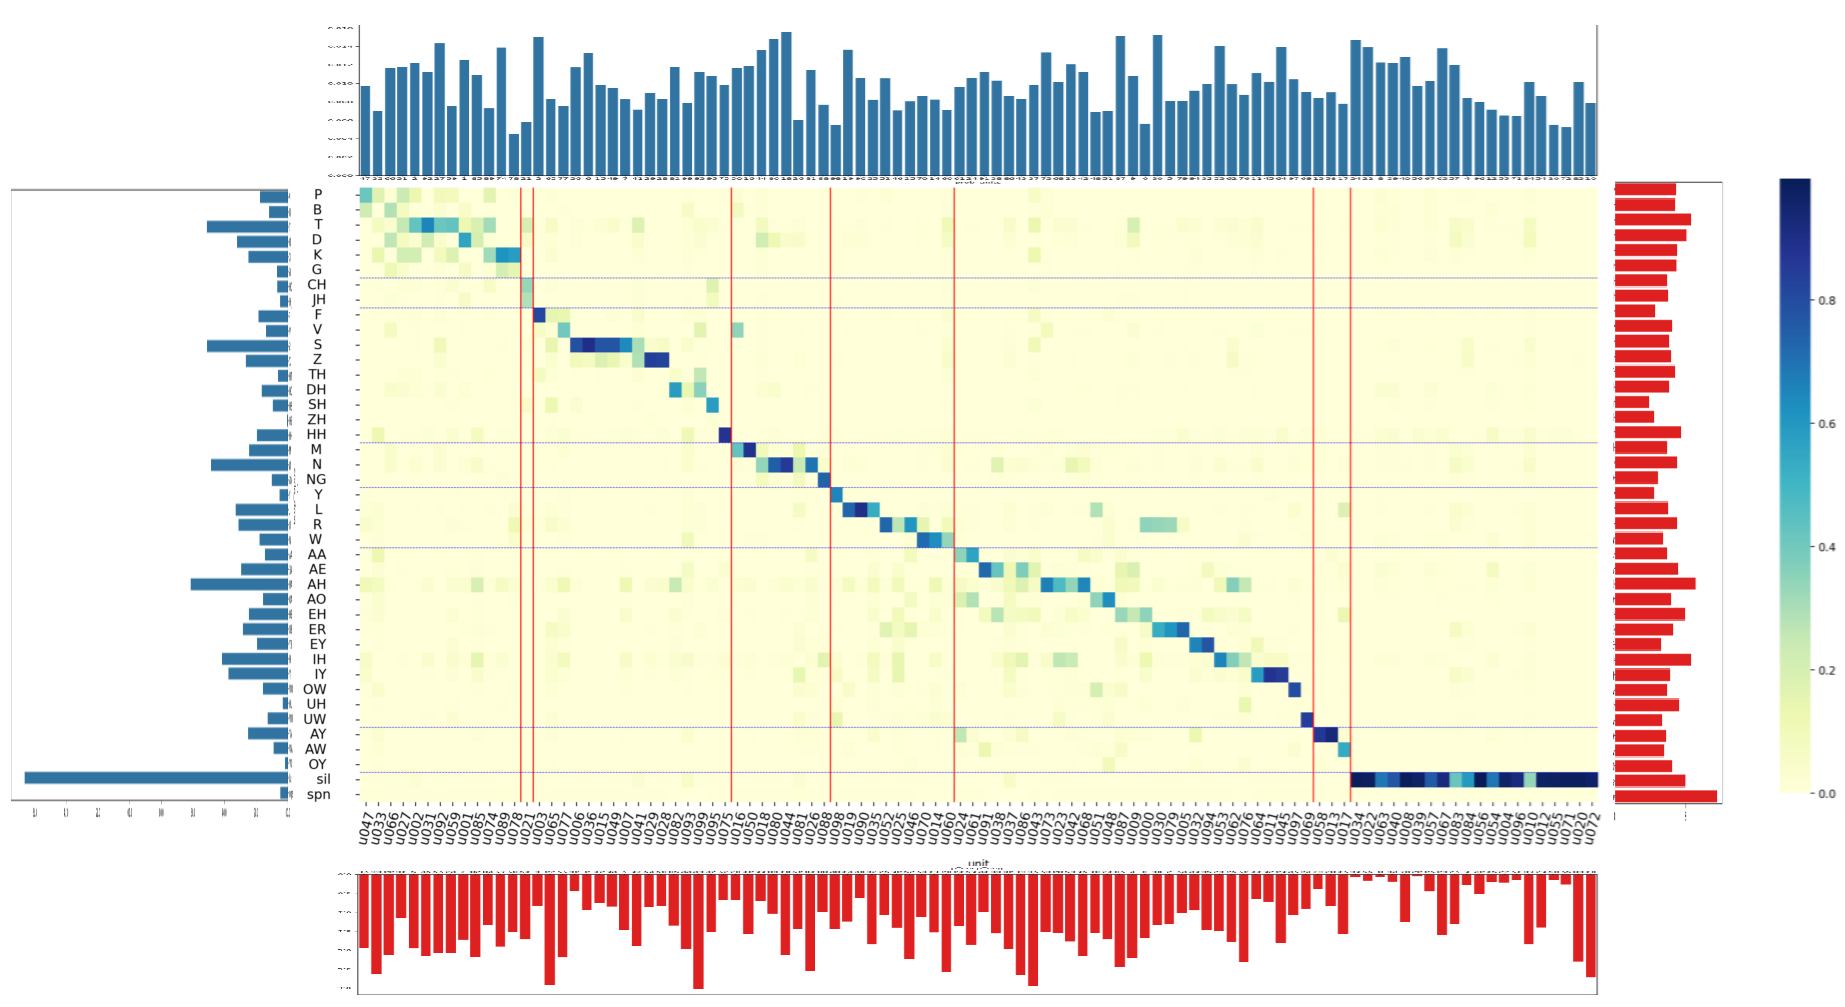
\includegraphics[width=1\linewidth]{figures/better__p_ph_given_un.png}\caption{HuBERT 100}\label{p_p_given_u-hub-100}
\end{figure}


}

  為了更直觀的了解模型離散單元與音素之間的對應關係,接下來的分析將把音素與單元的聯合分佈 \(p(p|u)\) 作圖呈現,如 \ref{p_p_given_u-hub-100} 所示。以下說明這張圖表的看法:

        橫軸是各單元,而縱軸是各音素,按照發音分組方式,輔音遵循國際音標的圖表排列,元音則按照 ARPABET (cite CMU Dict) 字母順序排列。由於離散單元編號本身並無特殊含義,因此當單元數太多時將省略。

        為了更好的看出各組別之間的關係,圖表上先將各組之間以橫線區分。按照語音學分組後,為了考慮單元之間的代表性,將每個單元都找出相對應最高機率的音素,接著將每個單元亦依照對應音素在縱軸的排列順序一一排列,若是遇到對應同一音素的兩種離散單元,則以 \(p(u|p) \) 由高至低排列。最後再橫軸上也以語音學分組區分。

        如此一來,便能夠呈現出一張由左上至右下的對應圖。這張圖在 (cite DinoSR) 等 paper 也有呈現。從圖中可以看出,用來編碼 sil 的 unit 其實佔據了不小的部分。

\setcounter{section}{4}

\section{分析結果}

\subsection{基於各自音位的分析}


\begin{table}[!htbp]
    \centering
    \begin{subtable}[t]{\textwidth}
        \centering
        \begin{tabular}{|c|c|c|c|c|c|} \hline
                        & 音位純度   & 分群純度   & 音位熵    & 離散單元熵  & PNMI   \\ \hline
            HuBERT      &     0.5256 &     0.3382 &    3.3152 &      3.8681 & 0.4993 \\ \hline    %% 1.6552 h
            Wav2vec 2.0 &     0.4006 &     0.2676 &    3.3152 &      3.8215 & 0.3706 \\ \hline    %% 1.2286 w
            CPC         &     0.5188 &     0.3812 &    3.3146 &      3.7918 & 0.4992 \\ \hline    %% 1.6545 c
            LogMel      &     0.3253 &     0.1473 &    3.3158 &      3.8630 & 0.2647 \\ \hline    %% 0.8776 l 
        \end{tabular}
        \caption{群數 = 50}
        \label{tab:ch3-clu050-phn}
    \end{subtable}

    \vspace{0.5cm}

    \begin{subtable}[t]{\textwidth}
        \centering
        \begin{tabular}{|c|c|c|c|c|c|} \hline
                        & 音位純度   & 分群純度   & 音位熵    & 離散單元熵  & PNMI   \\ \hline
            HuBERT      &     0.6097 &     0.2553 &    3.3152 &      4.5704 & 0.5786 \\ \hline    %% 1.9181 h
            Wav2vec 2.0 &     0.4877 &     0.2118 &    3.3152 &      4.5284 & 0.4596 \\ \hline    %% 1.5235 w
            CPC         &     0.5895 &     0.2674 &    3.3146 &      4.5034 & 0.5557 \\ \hline    %% 1.8418 c
            LogMel      &     0.3348 &     0.0931 &    3.3158 &      4.5591 & 0.2789 \\ \hline    %% 0.9247 l 
        \end{tabular}
        \caption{群數 = 100}
        \label{tab:ch3-clu100-phn}
    \end{subtable}

    \vspace{0.5cm}

    \begin{subtable}[t]{\textwidth}
        \centering
        \begin{tabular}{|c|c|c|c|c|c|} \hline
                        & 音位純度   & 分群純度   & 音位熵    & 離散單元熵  & PNMI   \\ \hline
            HuBERT      &     0.6474 &     0.1644 &    3.3152 &      5.2681 & 0.6289 \\ \hline    %% 2.0849 h
            Wav2vec 2.0 &     0.5427 &     0.1467 &    3.3152 &      5.2173 & 0.5188 \\ \hline    %% 1.7199 w
            CPC         &     0.6098 &     0.1789 &    3.3146 &      5.1885 & 0.5882 \\ \hline    %% 1.9497 c
            LogMel      &     0.3474 &     0.0569 &    3.3158 &      5.2322 & 0.2955 \\ \hline    %% 0.9798 l 
        \end{tabular}
        \caption{群數 = 200}
        \label{tab:ch3-clu200-phn}
    \end{subtable}

    \caption{不同群數在四種基石模型的音位分析數據}
    \label{tab:single-cluster-results}
\end{table}


  由表 \ref{tab:single-cluster-results} 中可以看出,分群的群數愈多時,音位的純度確實有所上升,但這可能是犧牲分群純度得來的。因此再看 PNMI 的指標可以發現,整體離散單元和音位標註的相關性還是有所提升的。此外,從不同模型來觀察,HuBERT 的表現是四種語音表徵中最好的,一定程度上可以證實 HuBERT 在找出語音中有意義單位上的效能,及其為什麼無文字架構通常以 HuBERT 作為抽取語音離散表徵的模型。

\textcolor{red}{(討論太少應增加尤應增加舉例分析(某一 phoneme 對應到哪些 unit,它們如何分散或集中,不是只看平均值))}

\subsection{基於語音學及其音位分類的分析}


\begin{table}[!htbp]
    \centering
    \begin{subtable}[t]{\textwidth}
        \centering
        \begin{tabular}{|c|c|c|c|c|c|} \hline
                        & 標註純度   & 分群純度   & 標註熵    & 離散單元熵  & NMI    \\ \hline
            HuBERT      &     0.7466 &     0.1422 &    1.7530 &      3.8681 & 0.5742 \\ \hline    %% h  1.0065
            Wav2vec 2.0 &     0.6913 &     0.1570 &    1.7530 &      3.8215 & 0.4682 \\ \hline    %% w  0.8208
            CPC         &     0.7418 &     0.1953 &    1.7530 &      3.7918 & 0.5644 \\ \hline    %% c  0.9894
            LogMel      &     0.5980 &     0.0953 &    1.7530 &      3.8630 & 0.3403 \\ \hline    %% l  0.5966 
        \end{tabular}
        \caption{群數 = 50}
        \label{tab:ch3-clu050-pcls}
    \end{subtable}

    \vspace{0.2cm}

    \begin{subtable}[t]{\textwidth}
        \centering
        \begin{tabular}{|c|c|c|c|c|c|} \hline
                        & 標註純度   & 分群純度   & 標註熵    & 離散單元熵  & NMI    \\ \hline
            HuBERT      &     0.7804 &     0.0856 &    1.7530 &      4.5704 & 0.6148 \\ \hline    %% h  1.0778
            Wav2vec 2.0 &     0.7219 &     0.0889 &    1.7530 &      4.5284 & 0.5252 \\ \hline    %% w  0.9207
            CPC         &     0.7790 &     0.0997 &    1.7530 &      4.5034 & 0.6046 \\ \hline    %% c  1.0599
            LogMel      &     0.6032 &     0.0567 &    1.7530 &      4.5591 & 0.3512 \\ \hline    %% l  0.6157 
        \end{tabular}
        \caption{群數 = 100}
        \label{tab:ch3-clu100-pcls}
    \end{subtable}

    \vspace{0.2cm}

    \begin{subtable}[t]{\textwidth}
        \centering
        \begin{tabular}{|c|c|c|c|c|c|} \hline
                        & 標註純度   & 分群純度   & 標註熵    & 離散單元熵  & NMI    \\ \hline
            HuBERT      &     0.8004 &     0.0464 &    1.7530 &      5.2681 & 0.6563 \\ \hline    %% h  1.1504
            Wav2vec 2.0 &     0.7490 &     0.0527 &    1.7530 &      5.2173 & 0.5671 \\ \hline    %% w  0.9941
            CPC         &     0.7947 &     0.0644 &    1.7530 &      5.1885 & 0.6345 \\ \hline    %% c  1.1123
            LogMel      &     0.6107 &     0.0335 &    1.7530 &      5.2322 & 0.3652 \\ \hline    %% l  0.6401 
        \end{tabular}
        \caption{群數 = 200}
        \label{tab:ch3-clu200-pcls}
    \end{subtable}

    \caption{不同群數在四種基石模型按照語音學類別的分析數據}
    \label{tab:single-cluster-phonetype-results}
\end{table}


  將表 \ref{tab:single-cluster-phonetype-results} 與音位的表 \ref{tab:single-cluster-results} 進行比較,能看出音位數據表現的趨勢,也能在語音類別中看出來。然而,由於語音類別數明顯少於音位的種類數,因此語音類別標註的純度相較音位會較高。

\textcolor{red}{同樣太少討論,應增加尤其已有 3.3 的分類,尤可依據其 3.3 的類來分析}

\section{本章總結}

  本章節探討以音框為單位取出的語音離散表徵與對應的音位標註之間的關係,從分析結果中可以看到,HuBERT 模型的離散表徵確實與人類理解的語音單位「音位」之間具有最明顯的相似性,也進一步證明為何 HuBERT 是抽取語音離散表徵時最常使用的模型。

        然而,單一離散表徵僅能代表 10 或 20 毫秒的語音訊號,而音位的長度經常佔據不只一個離散表徵。因此,下一章節將進一步組合多個離散表徵成為符記,分析它們與音位之間的關係。
